\section{Evaluation}

    %Showcase the graph that summarizes the approach (scatter plot for different merge strategies)
    The above programs were run and tested for each merging strategy. 
    On merging, they were measured for the following: 
    \begin{itemize}
        \item Clock cycles utilized after merging. 
        \item Max resources that we require after merging. 
    \end{itemize}

    I also measured before merging, for each program, the clock cycles and adders required for each thread. 
    It is important to note that the total clock cycles represent the worst case scenario; if this program was run without merging. 

    The overall result was positive; it was possible to reduce or maintain the number of resources required, in addition to reducing the worst case number of clock cycles.
    Fig~\ref{Fig1} showcases the clock cycles saved from the worst case on merging: 
    %Insert graph here 
    \begin{figure}
        \centering
        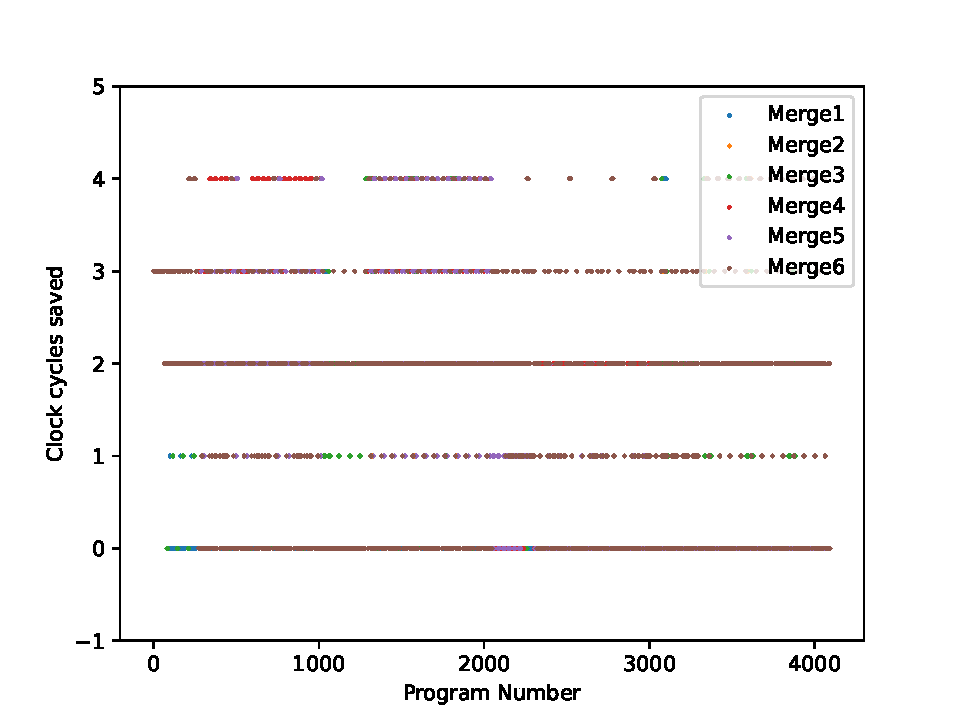
\includegraphics[scale=0.5]{m01.pdf}
        \caption{Scatter plot for each merging strategy, showing how many clock cyces were saved}
        \label{Fig1}
    \end{figure}

    I noticed that for each program, the clock cycles saved is at least zero.
    This shows us that at least merging does not result in total clock cycles required to be more than the original program. 
    The reason for this is quite intuitive; merging is equivalent to saying one thread executes first, followed by the second.
    Hence, naturally, the clock cycles will be bounded by the worst case before merging. 

    What is interesting however, is that the clock cycles are better than the worst case in almost 70percent of the programs that were considered after merging. 
    Fig~\ref{Fig2} shows the count of programs where (irrespective of how we merge) we save clock cycles on merge.  
    
        %inser graph here of clk_count 
        \begin{figure}
            \centering
            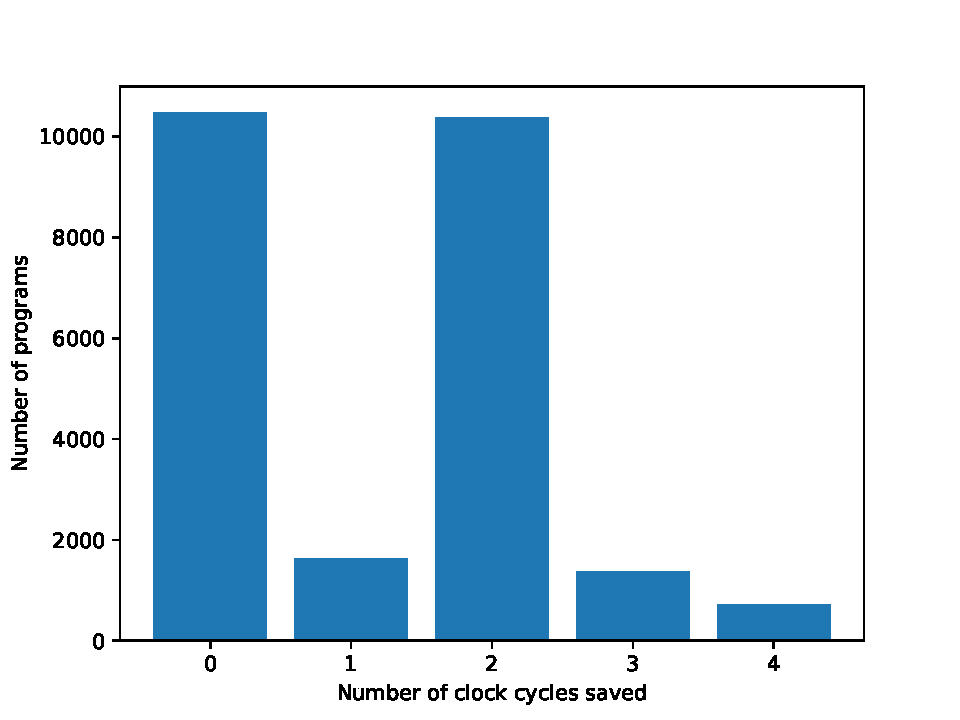
\includegraphics[scale=0.5]{clk_count.pdf}
            \caption{Count of programs after merging for the number of clock cycles saved.}
            \label{Fig2}
        \end{figure}
    
    
    This shows us a promise that merging indeed may not be detrimental to number of clock cycles; there will exist some merging that helps us save clock cycles in most cases.

    When it comes to resources, Fig~\ref{Fig3} showcases the resources saved (in comparison to pre-merge the amount of resources required).
    I noticed with the scatter plot that, once again, the amount of resources required is bounded by the amount required pre-merge. 
    What is interesting however, is that resources are saved, even though the scheduling algorithm is greedy, assuming infinte resources.
    This occured as adding additional memory dependency edges implicitly added dependency edges between the addition action too (this occurs due to Read-Write or Write-Read dependency edges). 
    \begin{figure}
        \centering
        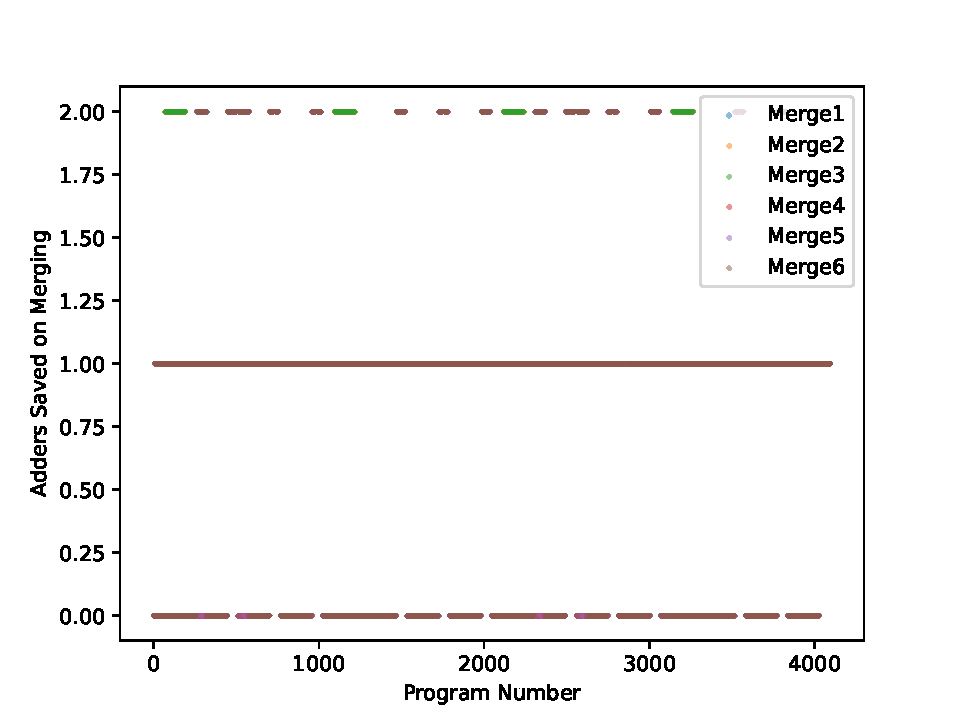
\includegraphics[scale=0.5]{m02.pdf}
        \caption{Scatter plot for each merging strategy, showing how many adders were saved}
        \label{Fig3}
    \end{figure}
    
    Fig~\ref{Fig4} shows us the count of programs (irrespective of how we merge) for the amount of resources we saved on merging.
    Once again, for most cases, some form of merging saved resources. 
    This is promising; as this shows us that resource constraints can be addressed by an optimization which just merges threads. 
    \begin{figure}
        \centering
        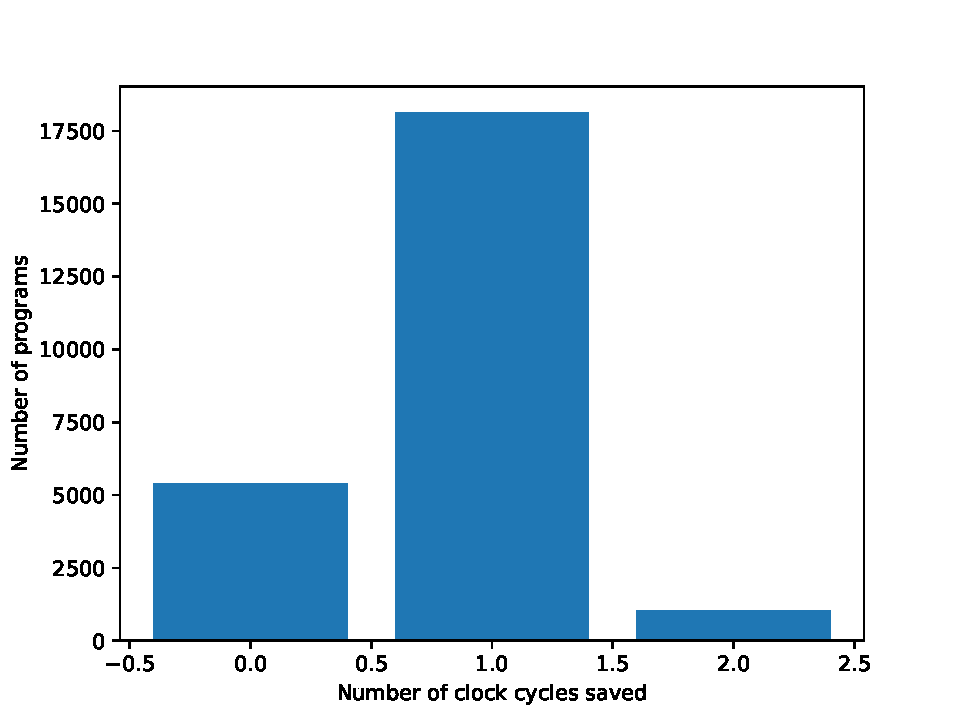
\includegraphics[scale=0.5]{add_count.pdf}
        \caption{Count of programs after merging for the number adders saved.}
        \label{Fig4}
    \end{figure}

    Our testing was done with 6 possible mergings; which interleave program statements. 
    Normally, merging is done by sequentializing a thread after another. 
    But here, merging was performed on a more fine grained level. 
    Is this useful though? Can we do away with just simple thread level merging? 
    Turns out, interleaving forms of merging do help us; more clock cycles as well as more resources can be saved.

    Fig~\ref{Fig5} showcases for each merging strategy, the amount of programs that benefited in saving clock cycles.
    We note that the trend is same, overall around 70percent of the programs benefit by merging; saving clock cycles.
    \begin{figure}
        \centering
        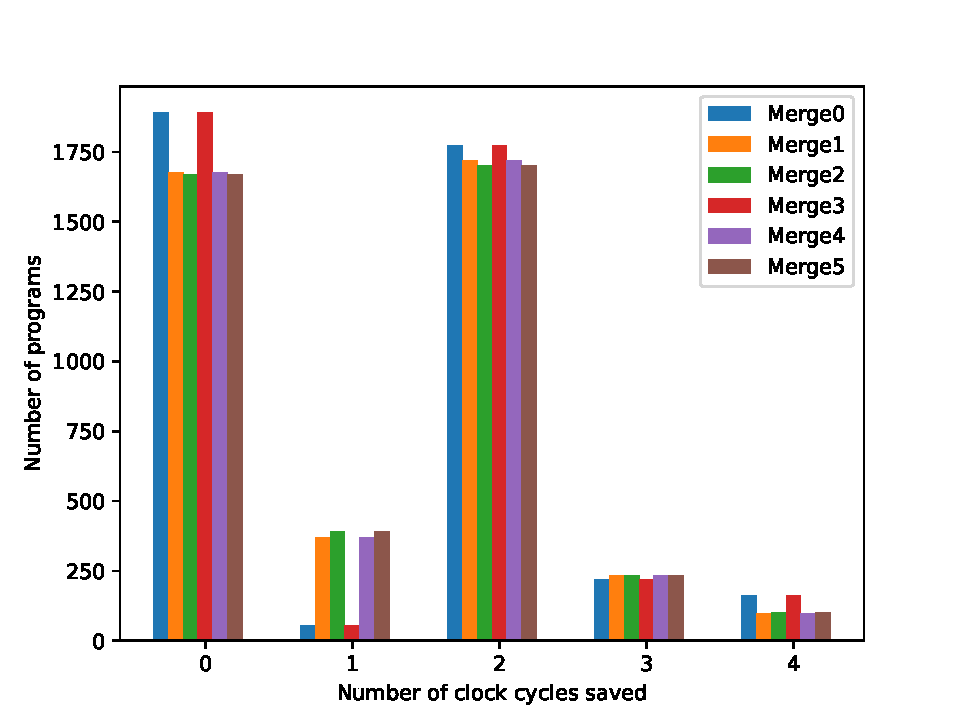
\includegraphics[scale=0.5]{per_merge_clck_saved.pdf}
        \caption{Graph showing for each merging strategy, the number of programs where merging saved clock cycles.}
        \label{Fig5}
    \end{figure}
    
    Fig~\ref{Fig6} showcases for each merging strategy, the amount of programs that benefited in saving adders.
    We once again, note that in most cases, the amount of adders required after merging reduces at least by 1; irrespective of what merging strategy we use. 
    \begin{figure}
        \centering
        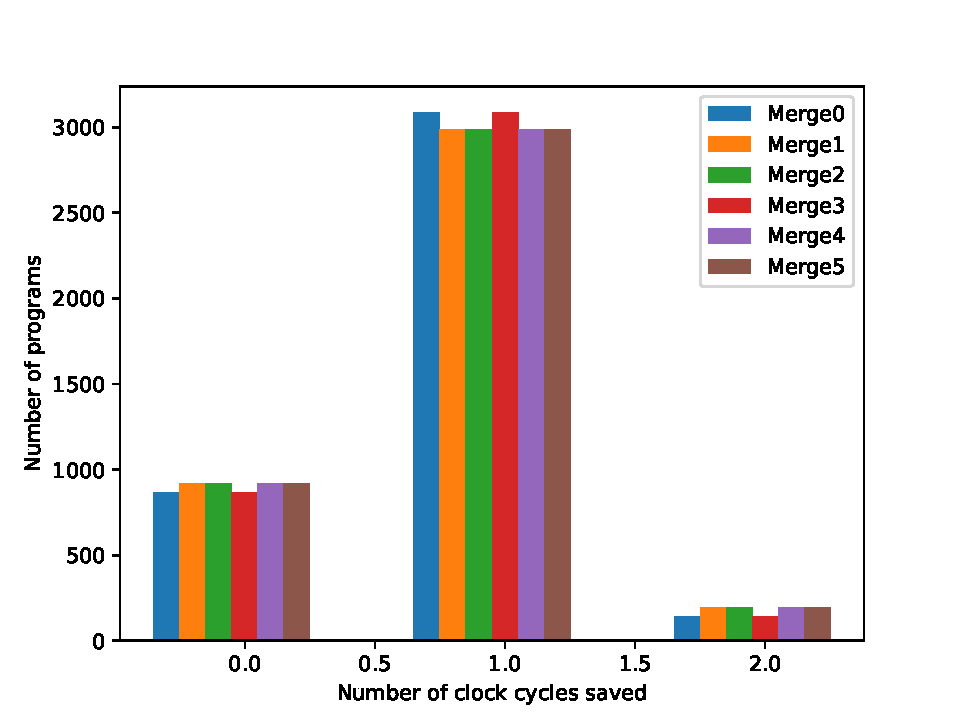
\includegraphics[scale=0.5]{per_merge_add_saved.pdf}
        \caption{Graph showing for each merging strategy, the number of programs where merging saved adders.}
        \label{Fig6}
    \end{figure}

    The above results show us that merging as an optimization is helpful in addressing the resource constraint problem.
    In addition, we do not detriment the overall clock cycles required for the program; this is always bounded by the worst case clock cycles of the original program.
    Moreover, in most cases, we even improve on this bound. 
    
    So far the above statistics does not indicate whether we require all forms of merging. 
    It is important to note that simple merging one thread after the other did not always result in the best resource usage and clock cycles.
    For instance, for the program in Fig~\ref{ex1}, the best merging optimization was interleaving t2's first statement after t1's first statement. Followed by t1's second statement and t2's second statement. 
    \begin{figure}
        \centering
        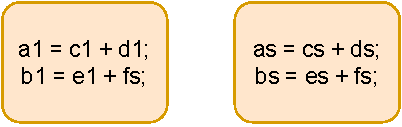
\includegraphics[scale=0.5]{Ex2.pdf}
        \caption{Program for which Merging by interleaving program statements results in a better schedule.}
        \label{ex1}
    \end{figure}

    The schedule for merging this way is given in Fig~\ref{ex1-schd}.
    The blue arrow represnt the memory dependency edges.
    The red circles represent the appropriate clock cycles when an action can be performed; as prescribed by greedy scheduling.
    The green boxes reprsent memory reads and blue boxes memory writes.
    The yellow arrow shows the order in which the two threads were merged.
    The overall schedule saved 2 clock cycles and 1 adder. 
    \begin{figure}
        \centering
        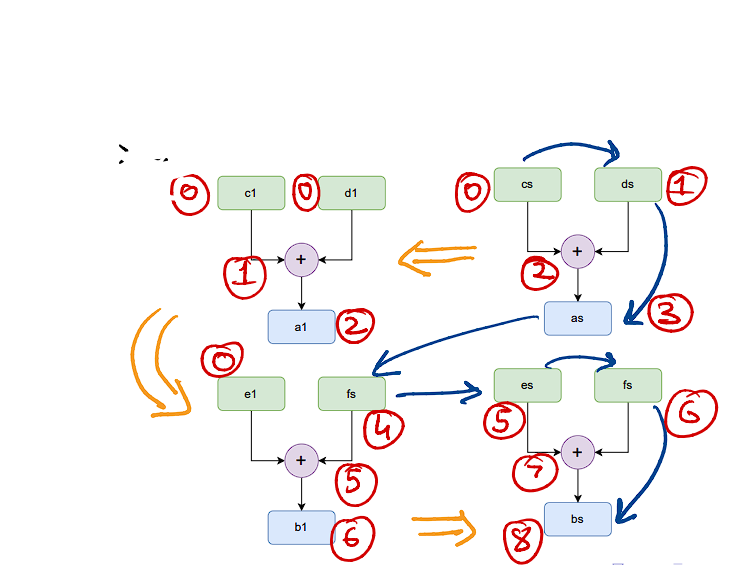
\includegraphics[scale=0.5]{Ex_schd.PNG}
        \caption{The schedule for merging in an interleaved fashion, giving us better schedule in comparison.}
        \label{ex1-schd}
    \end{figure}